\chapter{A Doença de Parkinson}
\section{Definição}

A DP é uma doença crônica, progressiva e degenerativa do sistema nervoso central, reconhecida principalmente por distúrbios motores como a bradicinesia, os tremores corporais em repouso e a rigidez corporal \cite{da2016aspectos}. A bradicinesia é a redução da movimentação, ou seja, o indivíduo consegue se movimentar porém lentamente. 

A DP é resultante da degeneração lenta, severa e irreparável dos neurônios dopaminérgicos da substância negra. Os neurônios dopaminérgicos são responsáveis pela produção de dopamina, um neurotransmissor fundamental para a gestão dos movimentos. Com a degeneração destes neurônios, a quantidade de dopamina é reduzida e, consequentemente, as mensagens nervosas para os músculos se tornam gradualmente mais lentas e desorganizadas. A substância negra localiza-se no mesencéfalo, parte intermediária do cérebro, conforme mostra a Figura ~\ref{substanciaNegra} \cite{eftaxias2015detection}.

\begin{figure}[!htb]
	\centering
	\includegraphics[width=0.8\textwidth]{figuras/subNegra.eps}
	\caption{Diagrama da substância negra, adaptado de \citeonline{figUm}.}
	\label{substanciaNegra}
\end{figure}

\section{Diagnóstico e Sintomas}
A DP afeta aproximadamente entre 1\% a 2\% da população mundial acima dos 65 anos, sendo que no Brasil atinge entorno de 3\% da população nesta faixa etária \cite{magalhaes2009descobrindo}. A idade é o único fator de risco conhecido. Segundo \citeonline{peixinho2006alteraccoes} a ocorrência de DP é rara antes dos 40 anos, aumenta após os 50 e tem maior probabilidade após os 70 anos. Porém a incidência da doença não está restrita somente a pessoas idosas, visto que 20\% dos casos são de pessoas com menos de 50 anos \cite{gago2014manual}. Não há consenso estabelecido, mas alguns estudos relacionam ser um pouco maior a ocorrência de DP no sexo masculino \cite{peixinho2006alteraccoes}.

O diagnóstico da DP é clínico, realizado normalmente por um neurologista, onde identifica-se a bradicinesia (lentidão dos movimentos) e pelo menos um de três outros sintomas \cite{gago2014manual}:
\begin{itemize}
	\item Tremor em repouso;
	\item Rigidez muscular;
	\item Instabilidade postural.
\end{itemize}

Outros exames também podem ser utilizados para confirmação da DP, como tomografia computadorizada e ressonância magnética cerebral, dentre outros a ser prescrito pelo médico responsável \cite{gago2014manual}.

Sobre os sintomas recorrentes da DP, os mesmos são associados a comunicação oral onde 90\% dos pacientes possuem problemas relacionados a fala, como gagueira, rouquidão, alteração ou enfraquecimento da voz \cite{zarzur2010laryngeal}. Também pode ocorrer alterações no sono, na memória além de depressão \cite{barbosa2005parkinsons}. Outro sintoma relevante é a demência que afeta cerca de 25\% dos pacientes com DP \cite{pamplona1996demencia}.

\subsection{Tratamento}
A DP não tem cura, consequentemente, os tratamentos disponíveis visam o controle dos sintomas para melhorar a qualidade de vida do paciente \cite{pamplona1996demencia}, com o objetivo de aumentar ao máximo sua autonomia e independência relacionada a atividades do cotidiano. Existem vários tipos de tratamentos, sendo essencial uma equipe multiprofissional, para atendimentos específicos relacionados a cada tipo de sintoma relacionado a doença \cite{saito2011doencca}.